\section{The Dataset}

\begin{frame}{Problem Setting}
	\begin{block}{}
		We define the multimodal input space as the Cartesian product of $P$ modality-specific input spaces:
		\[
		\mathcal{X} = \prod_{p=1}^{P} \mathcal{X}^{(p)},
		\]
		where each modality $\mathcal{X}^{(p)}$ may represent data from distinct sources.
	\end{block}
	
\end{frame}



\begin{frame}{Toadstool 2 Dataset}
\begin{block}{}
The dataset consists of video, sensor, and demographic data collected from 10 participants playing a Super Mario Bros.
\end{block}
		\begin{columns}[T] % Top alignment
		\begin{column}{0.4\textwidth}
			\includegraphics[width=\linewidth]{figures/toadstool.jpg}
			
		\end{column}
		\begin{column}{0.6\textwidth}

%		\vspace{0.5em}
		\centering
		\small
		\begin{tabular}{lcc}
		\toprule
		\textbf{Signal} & \textbf{Rate (Hz)} & \textbf{Channels} \\
		\midrule
		BVP  & 64 & 1      \\
		ACC  & 32 & 3 		\\
		EDA  & 4  & 1      \\
		HR   & 1  & 1      \\
		\bottomrule
		\end{tabular}
		
		\begin{figure}[htbp]
			\centering
			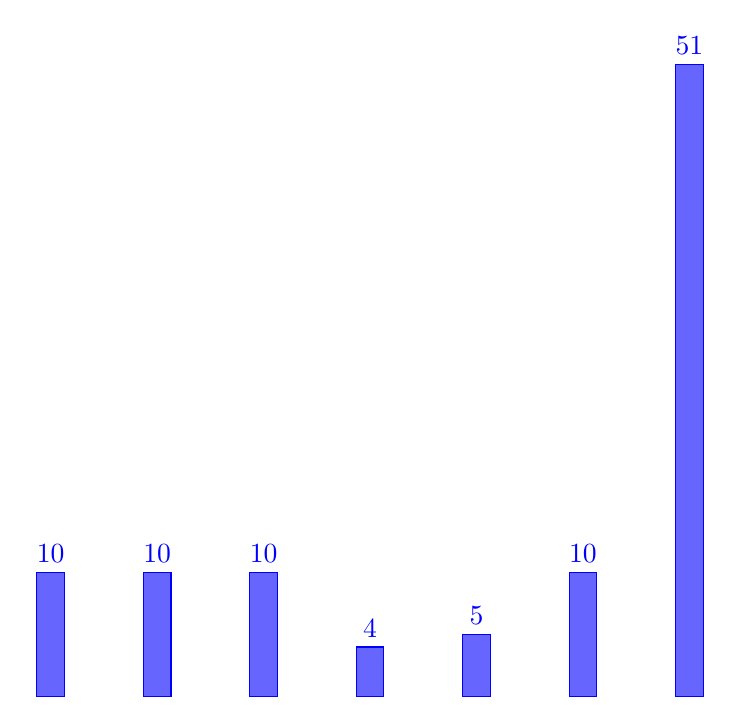
\begin{tikzpicture}
				\begin{axis}[
					width=\textwidth,
%					height=1cm,
					ybar,
					bar width=10pt,
					enlarge x limits=0.15,
					ylabel={\% of Samples},
					symbolic x coords={Disgust,Fear,Happy,Surprised,Sad,Anger,Neutral},
					xtick=data,
					axis x line=none,
					axis y line=none,
					tick style={draw=none},
					yticklabels={},
					nodes near coords,
					nodes near coords align={vertical},
					]
					\addplot+[fill=blue!60] coordinates {
						(Disgust,10) (Fear,10) (Happy,10) (Surprised,4) (Sad,5) (Anger,10) (Neutral,51)
					};
				\end{axis}
			\end{tikzpicture}
		\end{figure}


		\end{column}
	\end{columns}
\end{frame}


\begin{frame}{Total Class Distribution (\% of Samples)}
	\begin{center}
		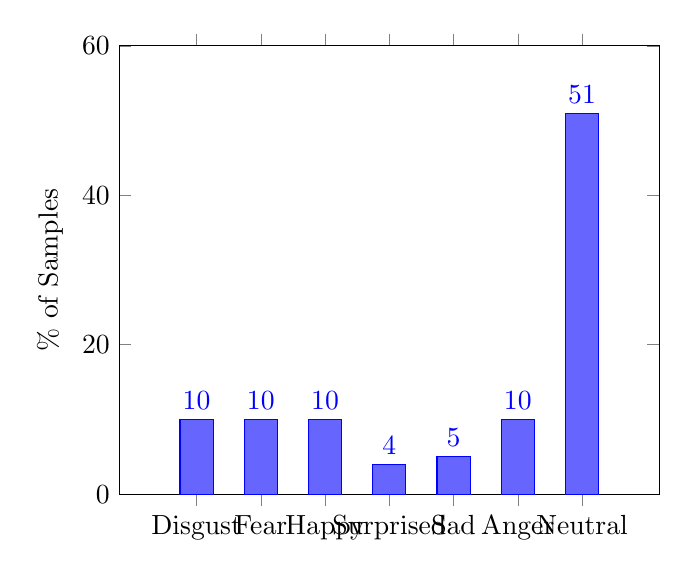
\begin{tikzpicture}
			\begin{axis}[
				ybar,
				bar width=12pt,
				enlarge x limits=0.2,
				ylabel={\% of Samples},
				symbolic x coords={Disgust,Fear,Happy,Surprised,Sad,Anger,Neutral},
				xtick=data,
				nodes near coords,
				nodes near coords align={vertical},
				ymin=0, ymax=60
				]
				\addplot+[fill=blue!60] coordinates {
					(Disgust,10) (Fear,10) (Happy,10) (Surprised,4) (Sad,5) (Anger,10) (Neutral,51)
				};
			\end{axis}
		\end{tikzpicture}
	\end{center}
	\note{Shows percentage breakdown of the seven emotion classes across all participants.}
\end{frame}

